%!TEX root = ../2019_7_Ozgumus_Semsi_Yigit.tex

\begingroup

This chapter presents the modifications applied to aforementioned approaches to improve the performance of the anomaly detection. All the discussed models measures its performance metric on well known datasets, such as CIFAR-10 \cite{cifar10} and SVHN \cite{Netzer2011ReadingDI}. The dataset used in this thesis presents additional challenges to this problem we aim to solve. The first section will introduce its dataset to the reader and will give examples. Next section will discuss the shortcomings of the previous approaches regarding the interpretation of the dataset and detection of the existent anomalies. Sections \ref{sec:encebgan} and \ref{sec:sencebgan} will explain the modified architecture and the significance of the changes.

\section{SEM Image Dataset}
\label{sec:sem}

Nanofibrous materials acquired increasingly significant demand from variety of fields in the Industry. It constitutes a foundation material for a lot of products including areas in medicine, filtration, sensors and manufacturing applications. \cite{carrera2016defect}. Despite the demand and continuous research development towards its production, manufacturing nanofibrous materials is still  challenge for scaled of mass production. Several techniques for producing nanofibers have been presented in the literature. \cite{carrera2016defect}. Electrospinning method is the focus of this anomaly detection task. It produces a structure which consists of filaments woven in without a certain pattern.  You can see one of the images of the material produced without any anomalies in figure \ref{fig:data_norm}.

\begin{figure}[h!]
	\centering
	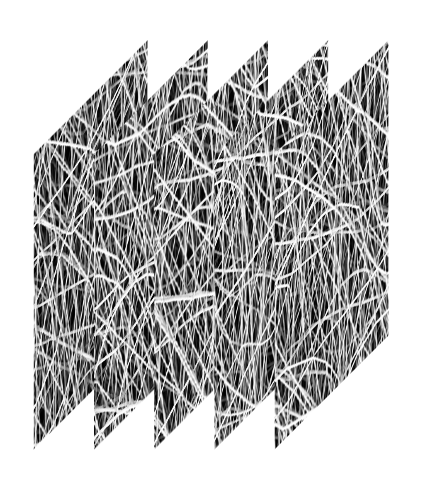
\includegraphics[width=1.0\textwidth]{dataset}
	\caption{Part of Training Dataset from the SEM Image Dataset \cite{sem}}
	\label{fig:data_norm}
\end{figure}


\begin{figure}[h!] \subfloat[Normal regions]{
		\begin{minipage}[c][1\width]{0.5\textwidth}
			\centering
			\fbox{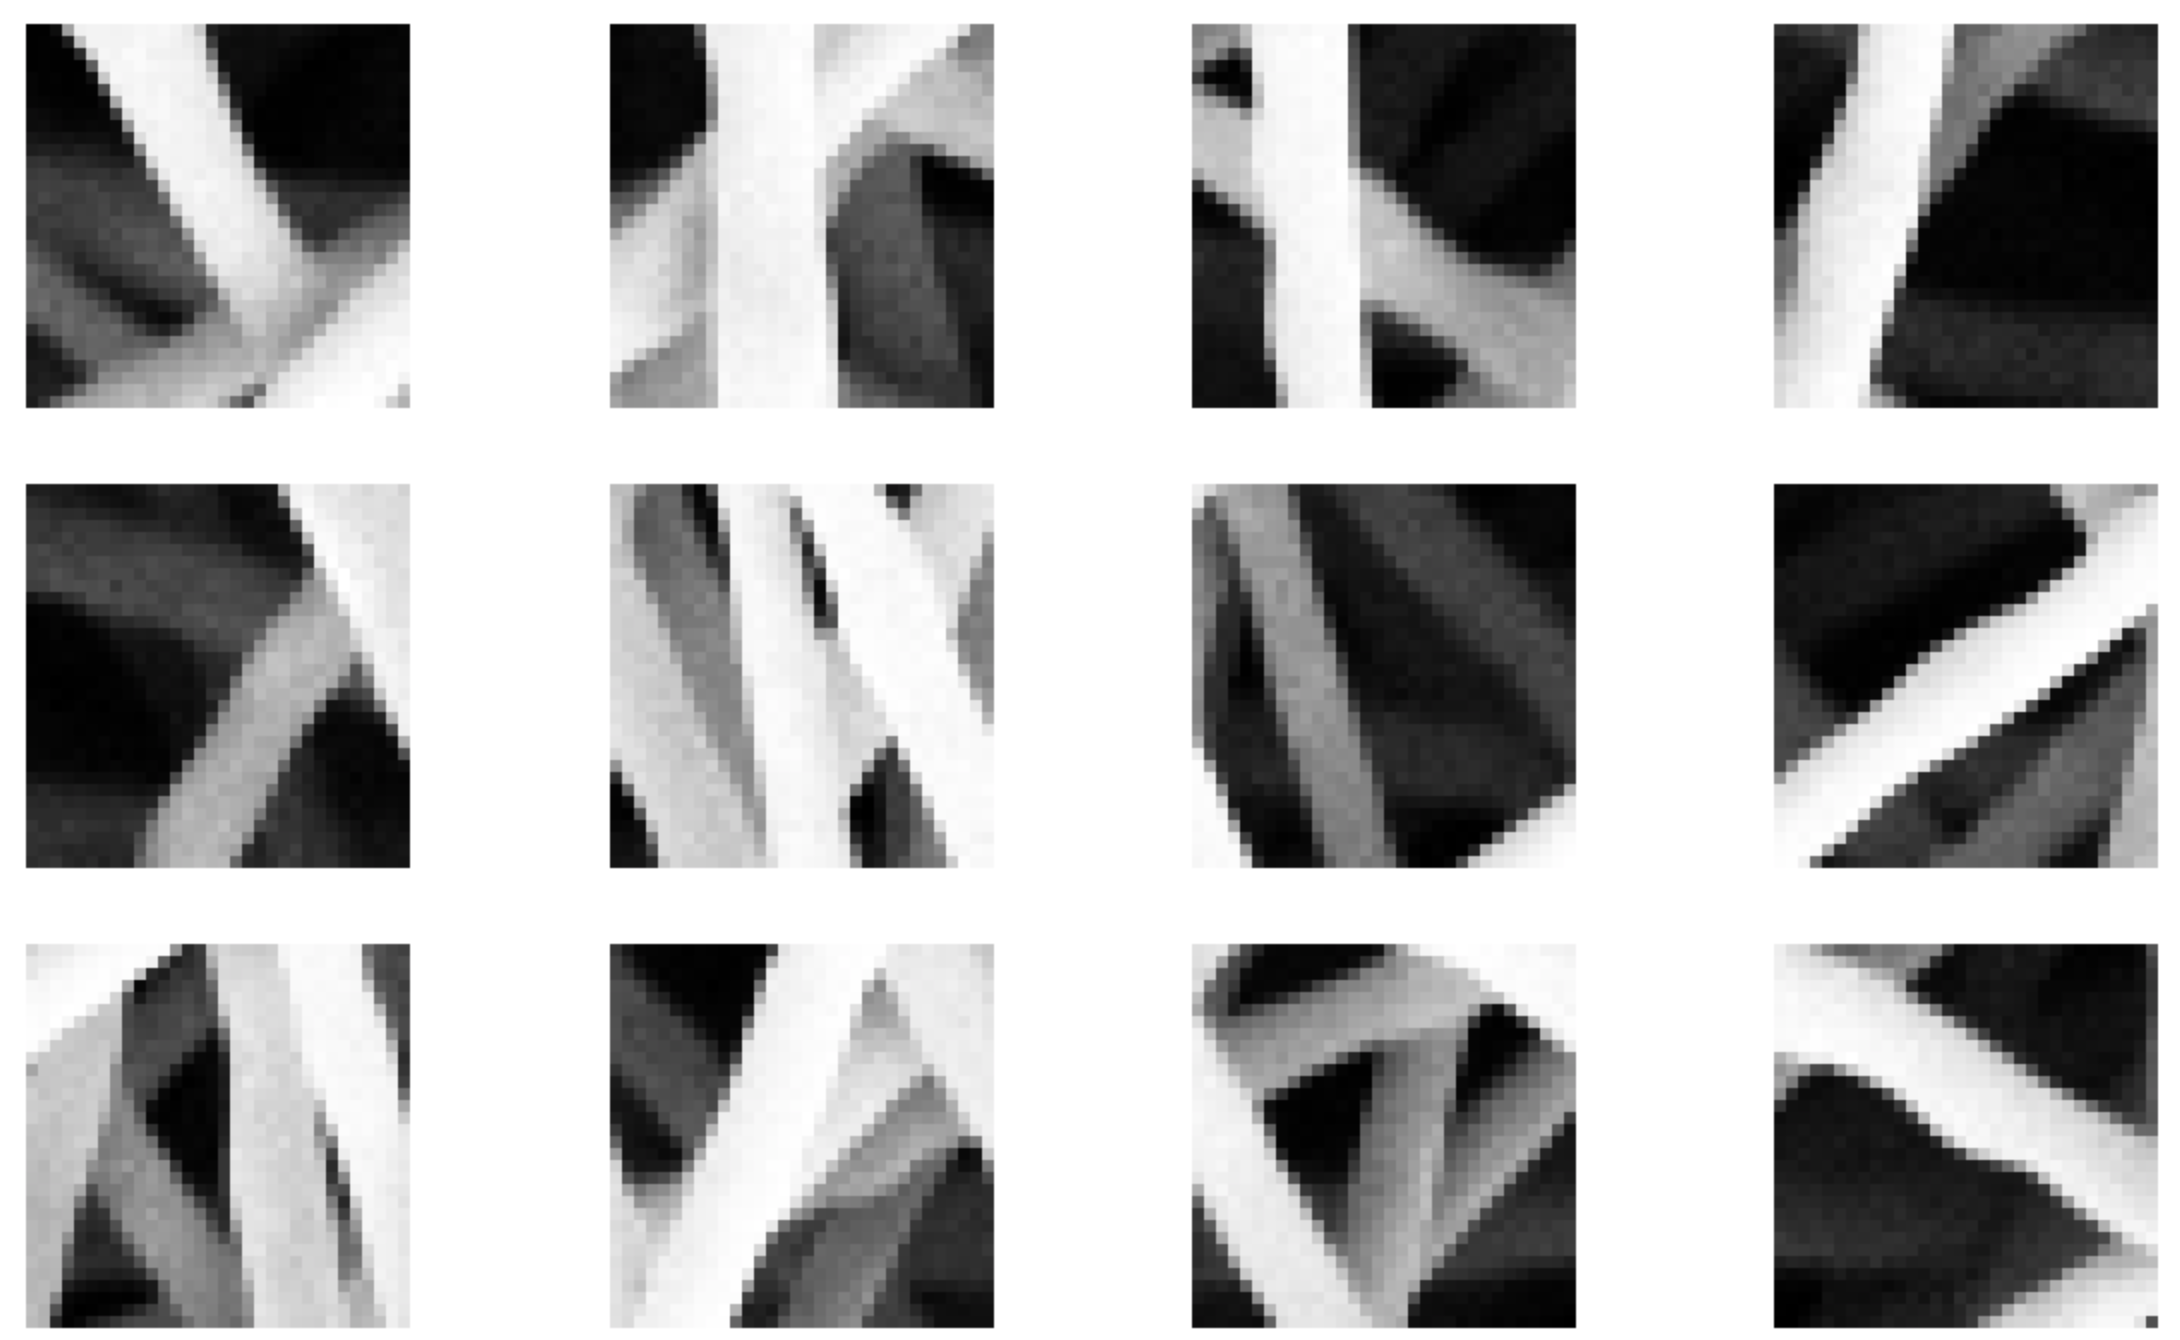
\includegraphics[width=1\textwidth]{sample_normal}}
	\end{minipage}}
	\hfill 	
	\subfloat[Anomalous regions]{
		\begin{minipage}[c][1\width]{0.5\textwidth}
			\centering
			\fbox{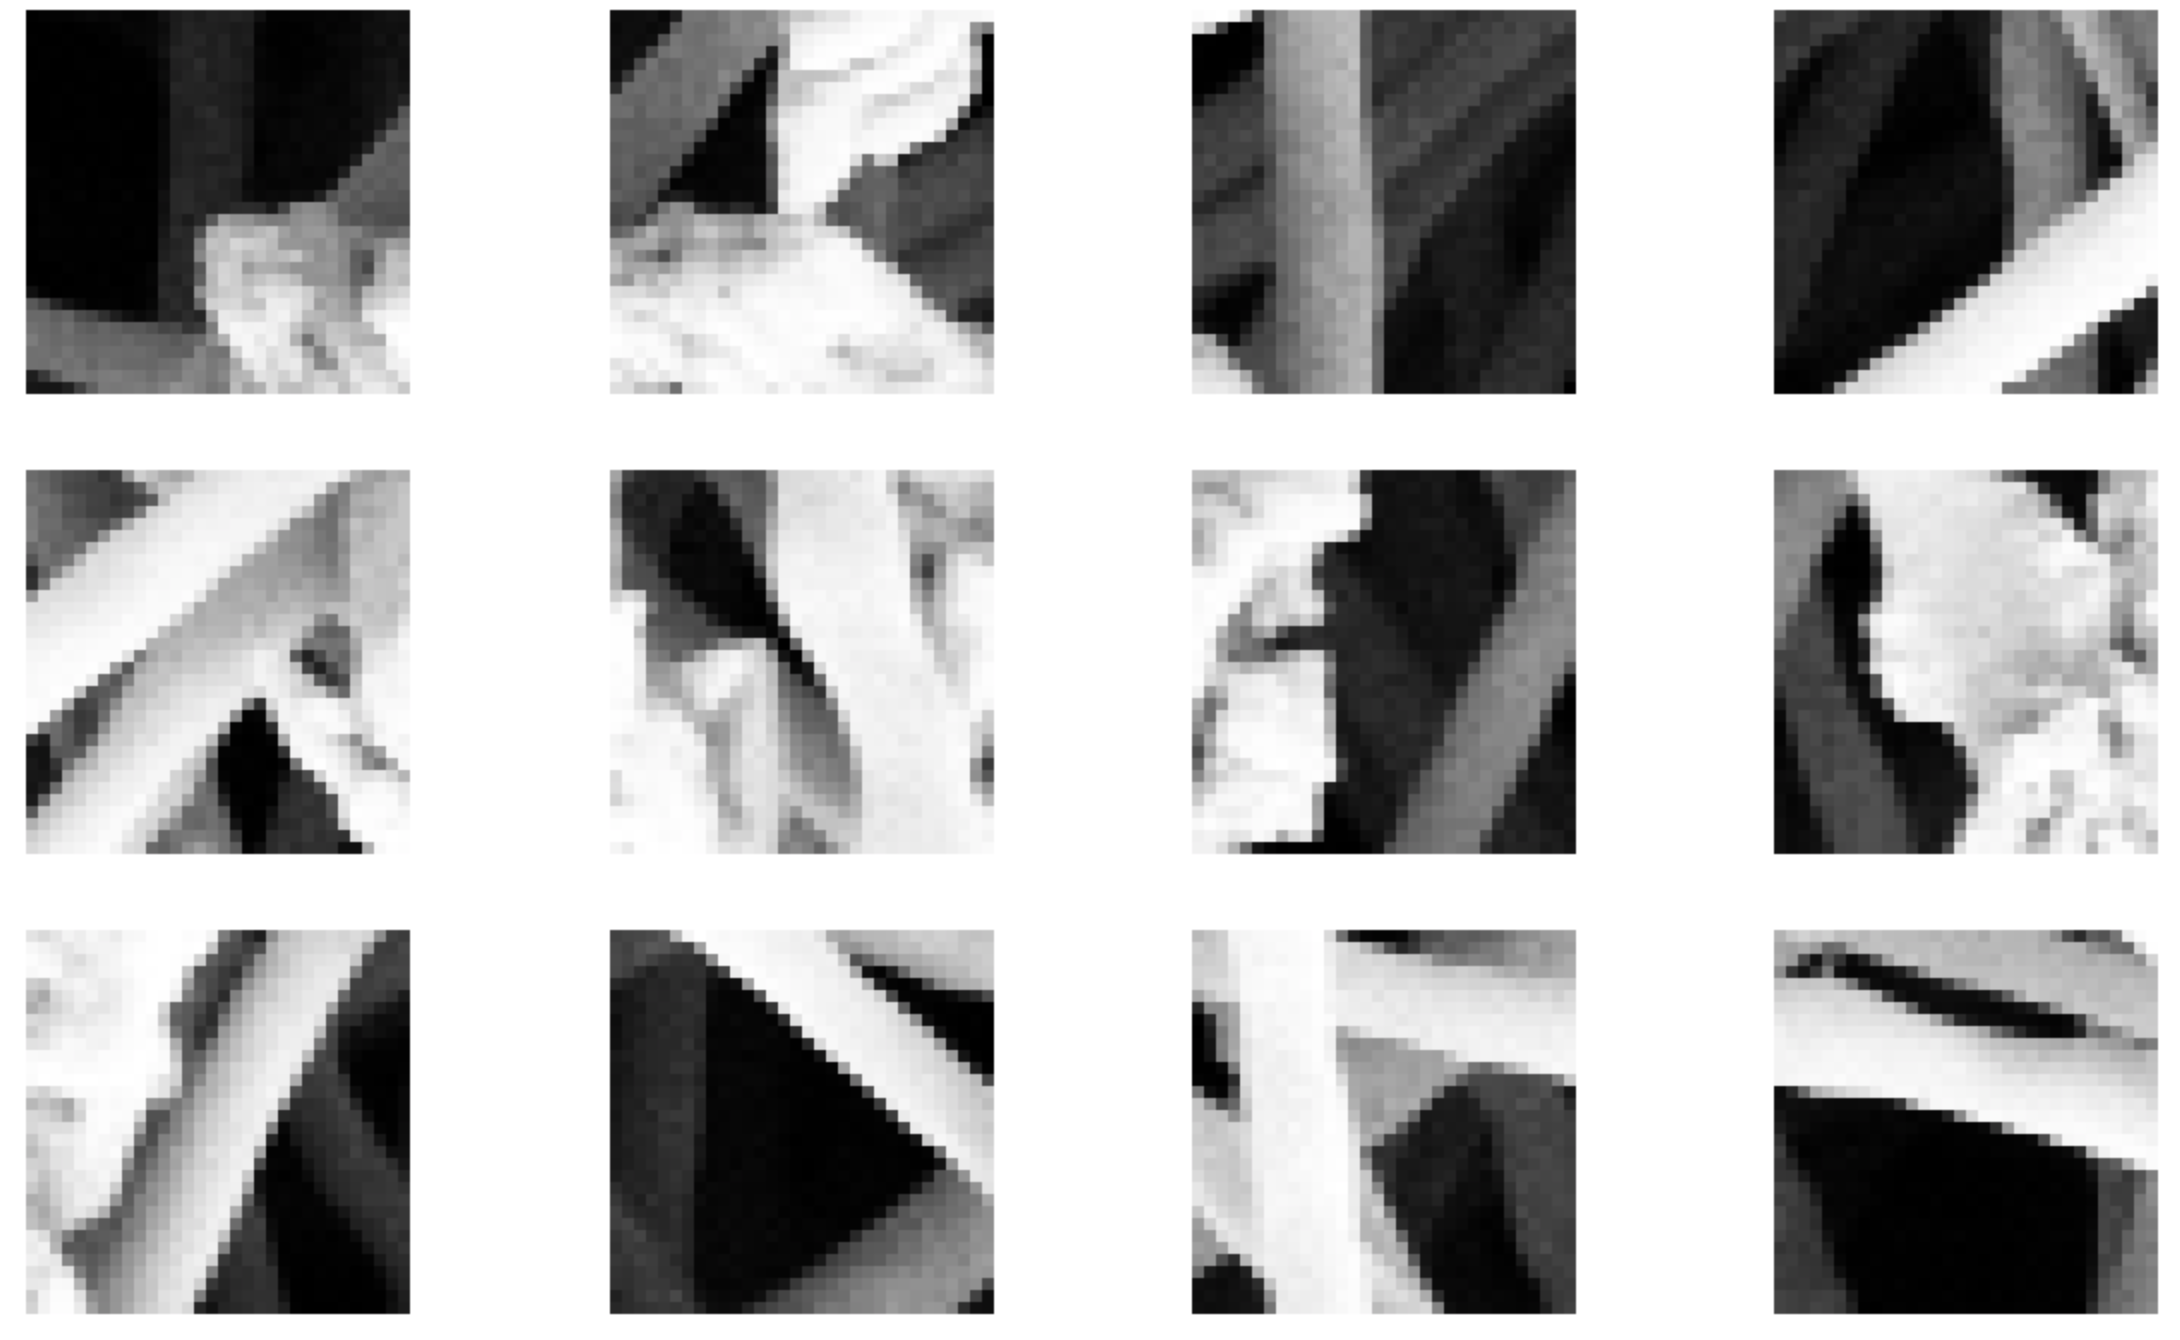
\includegraphics[width=1\textwidth]{sample_anomaly}}
	\end{minipage}}
	\caption{Normal and Anomalous region patches for the training and testing}
	\label{fig:data_samples}
\end{figure}

\section{Analysis of Aforementioned Approaches}
\label{sec:analysis_before}

\begin{figure}[h!]
	\centering
	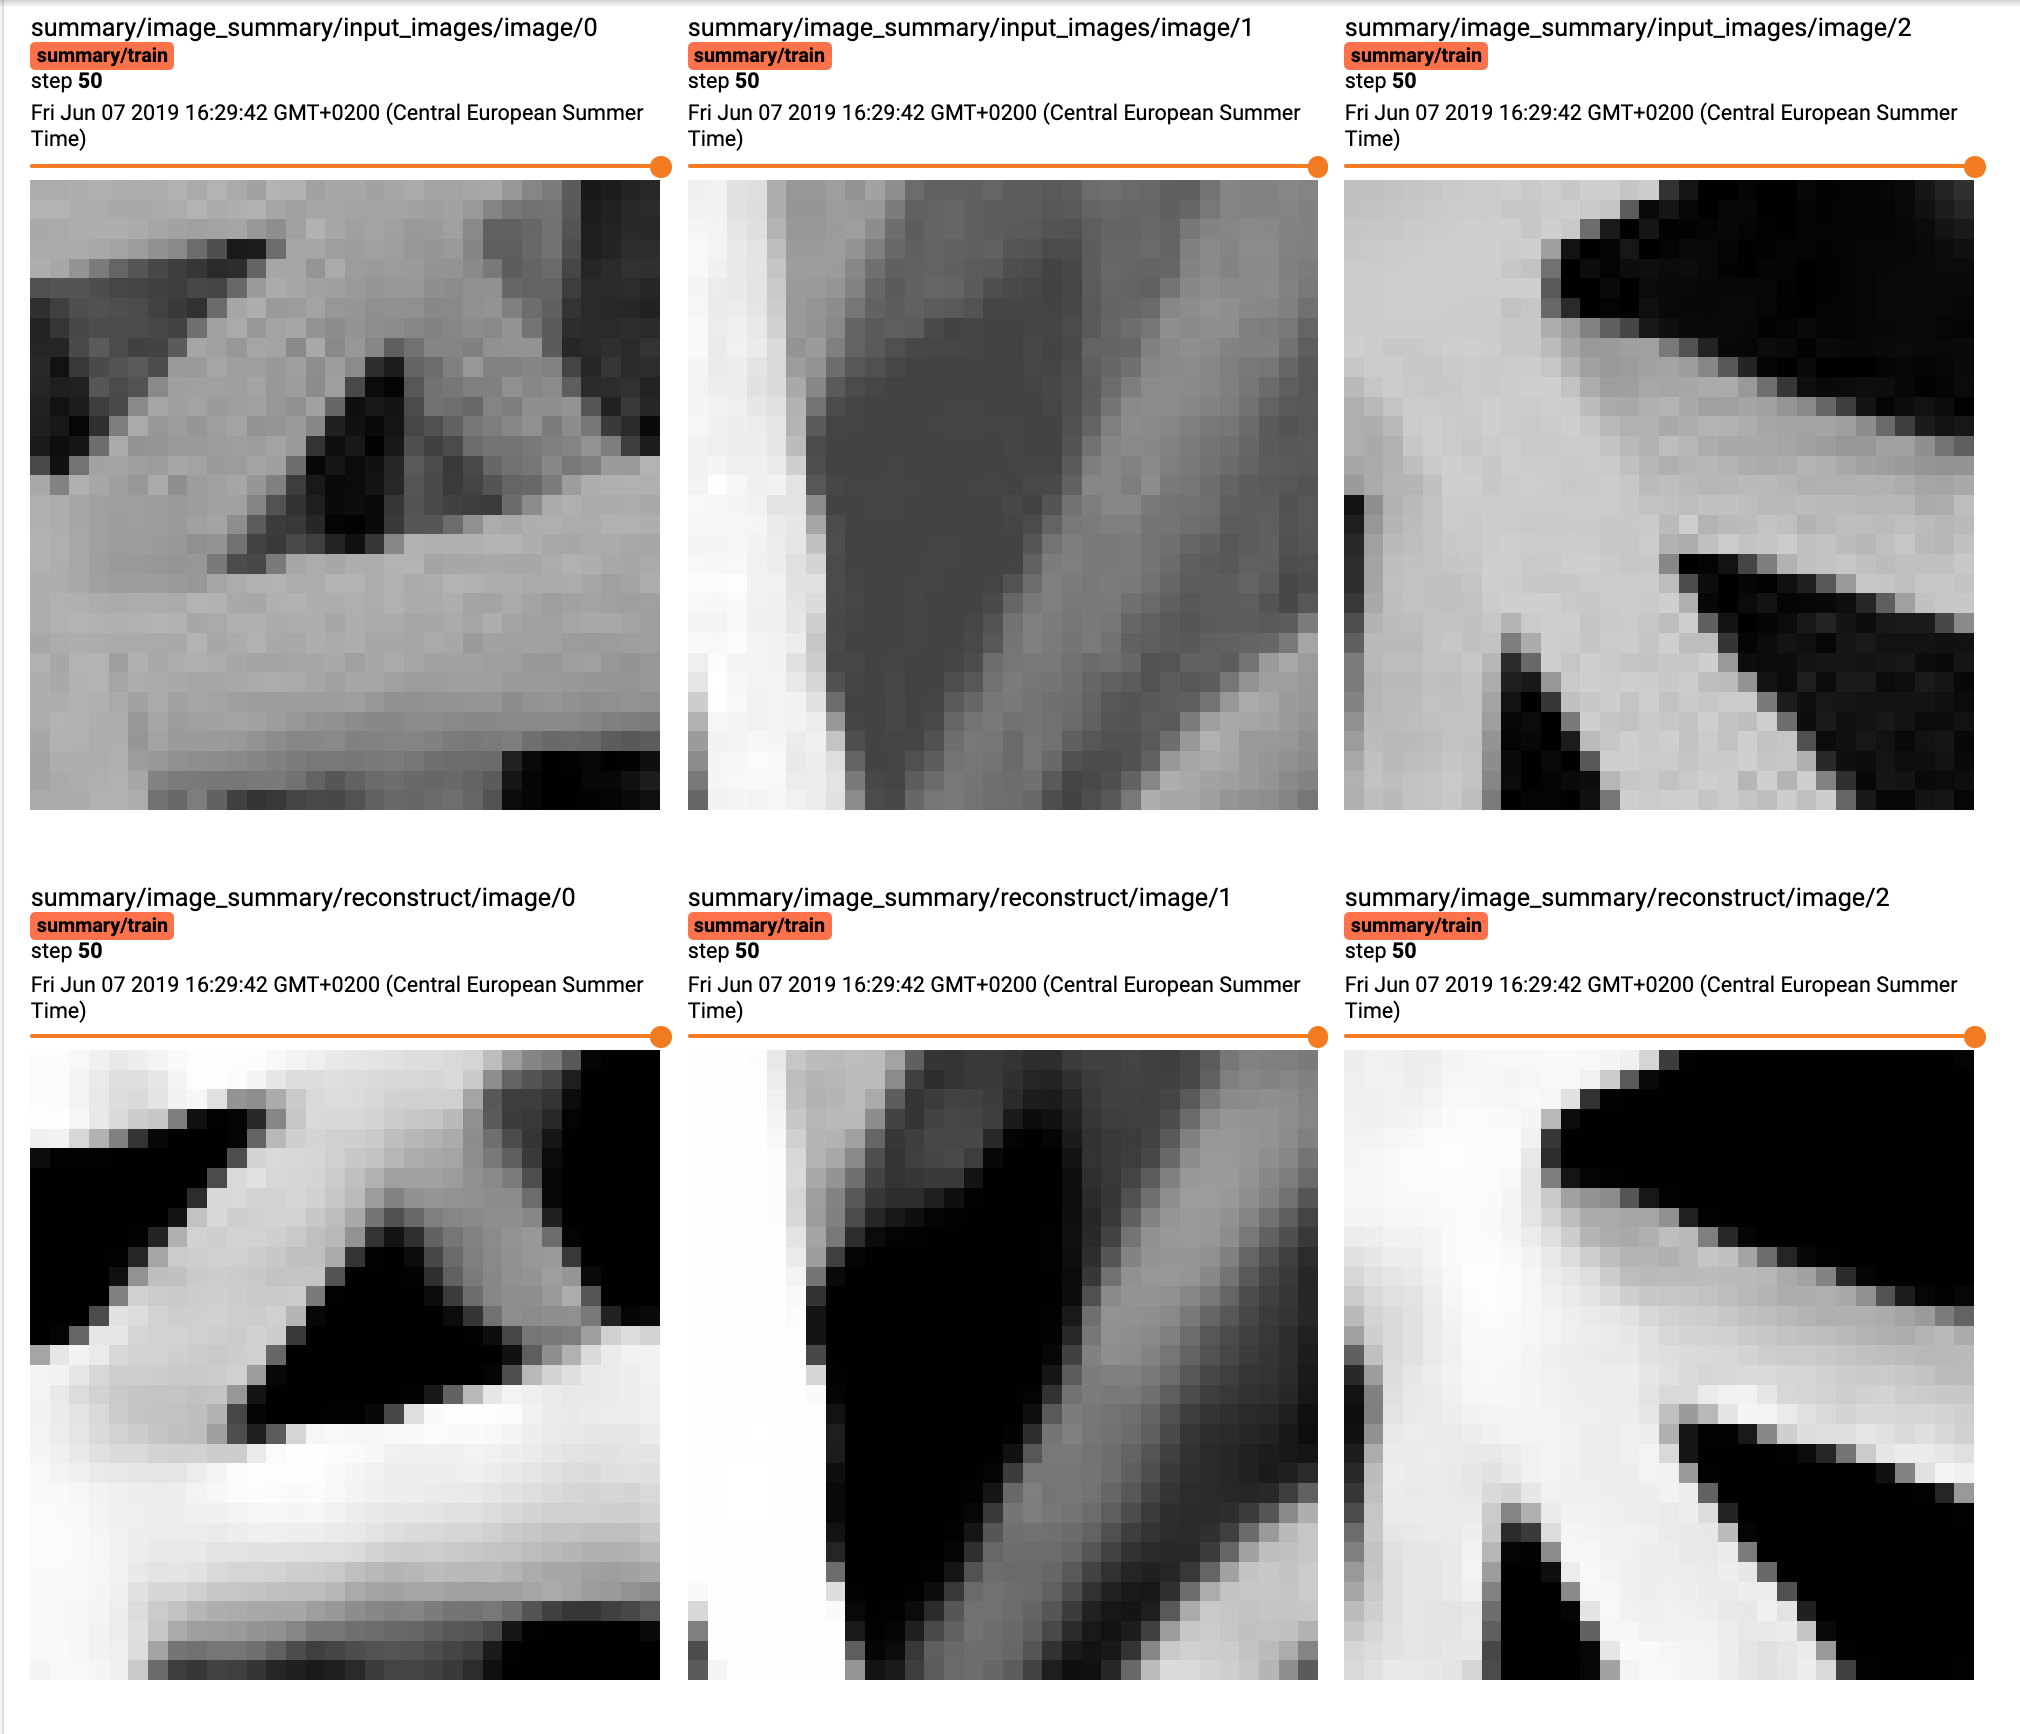
\includegraphics[width=0.75\textwidth]{reconstruct_ganomaly}
	\caption{SENCEBGAN Model Overview }
	\label{fig:sencebgan_model}
\end{figure}

\section{Encoded Energy Based Generative Adversarial Network}
\label{sec:encebgan}

\begin{figure}[h!]
	\centering
	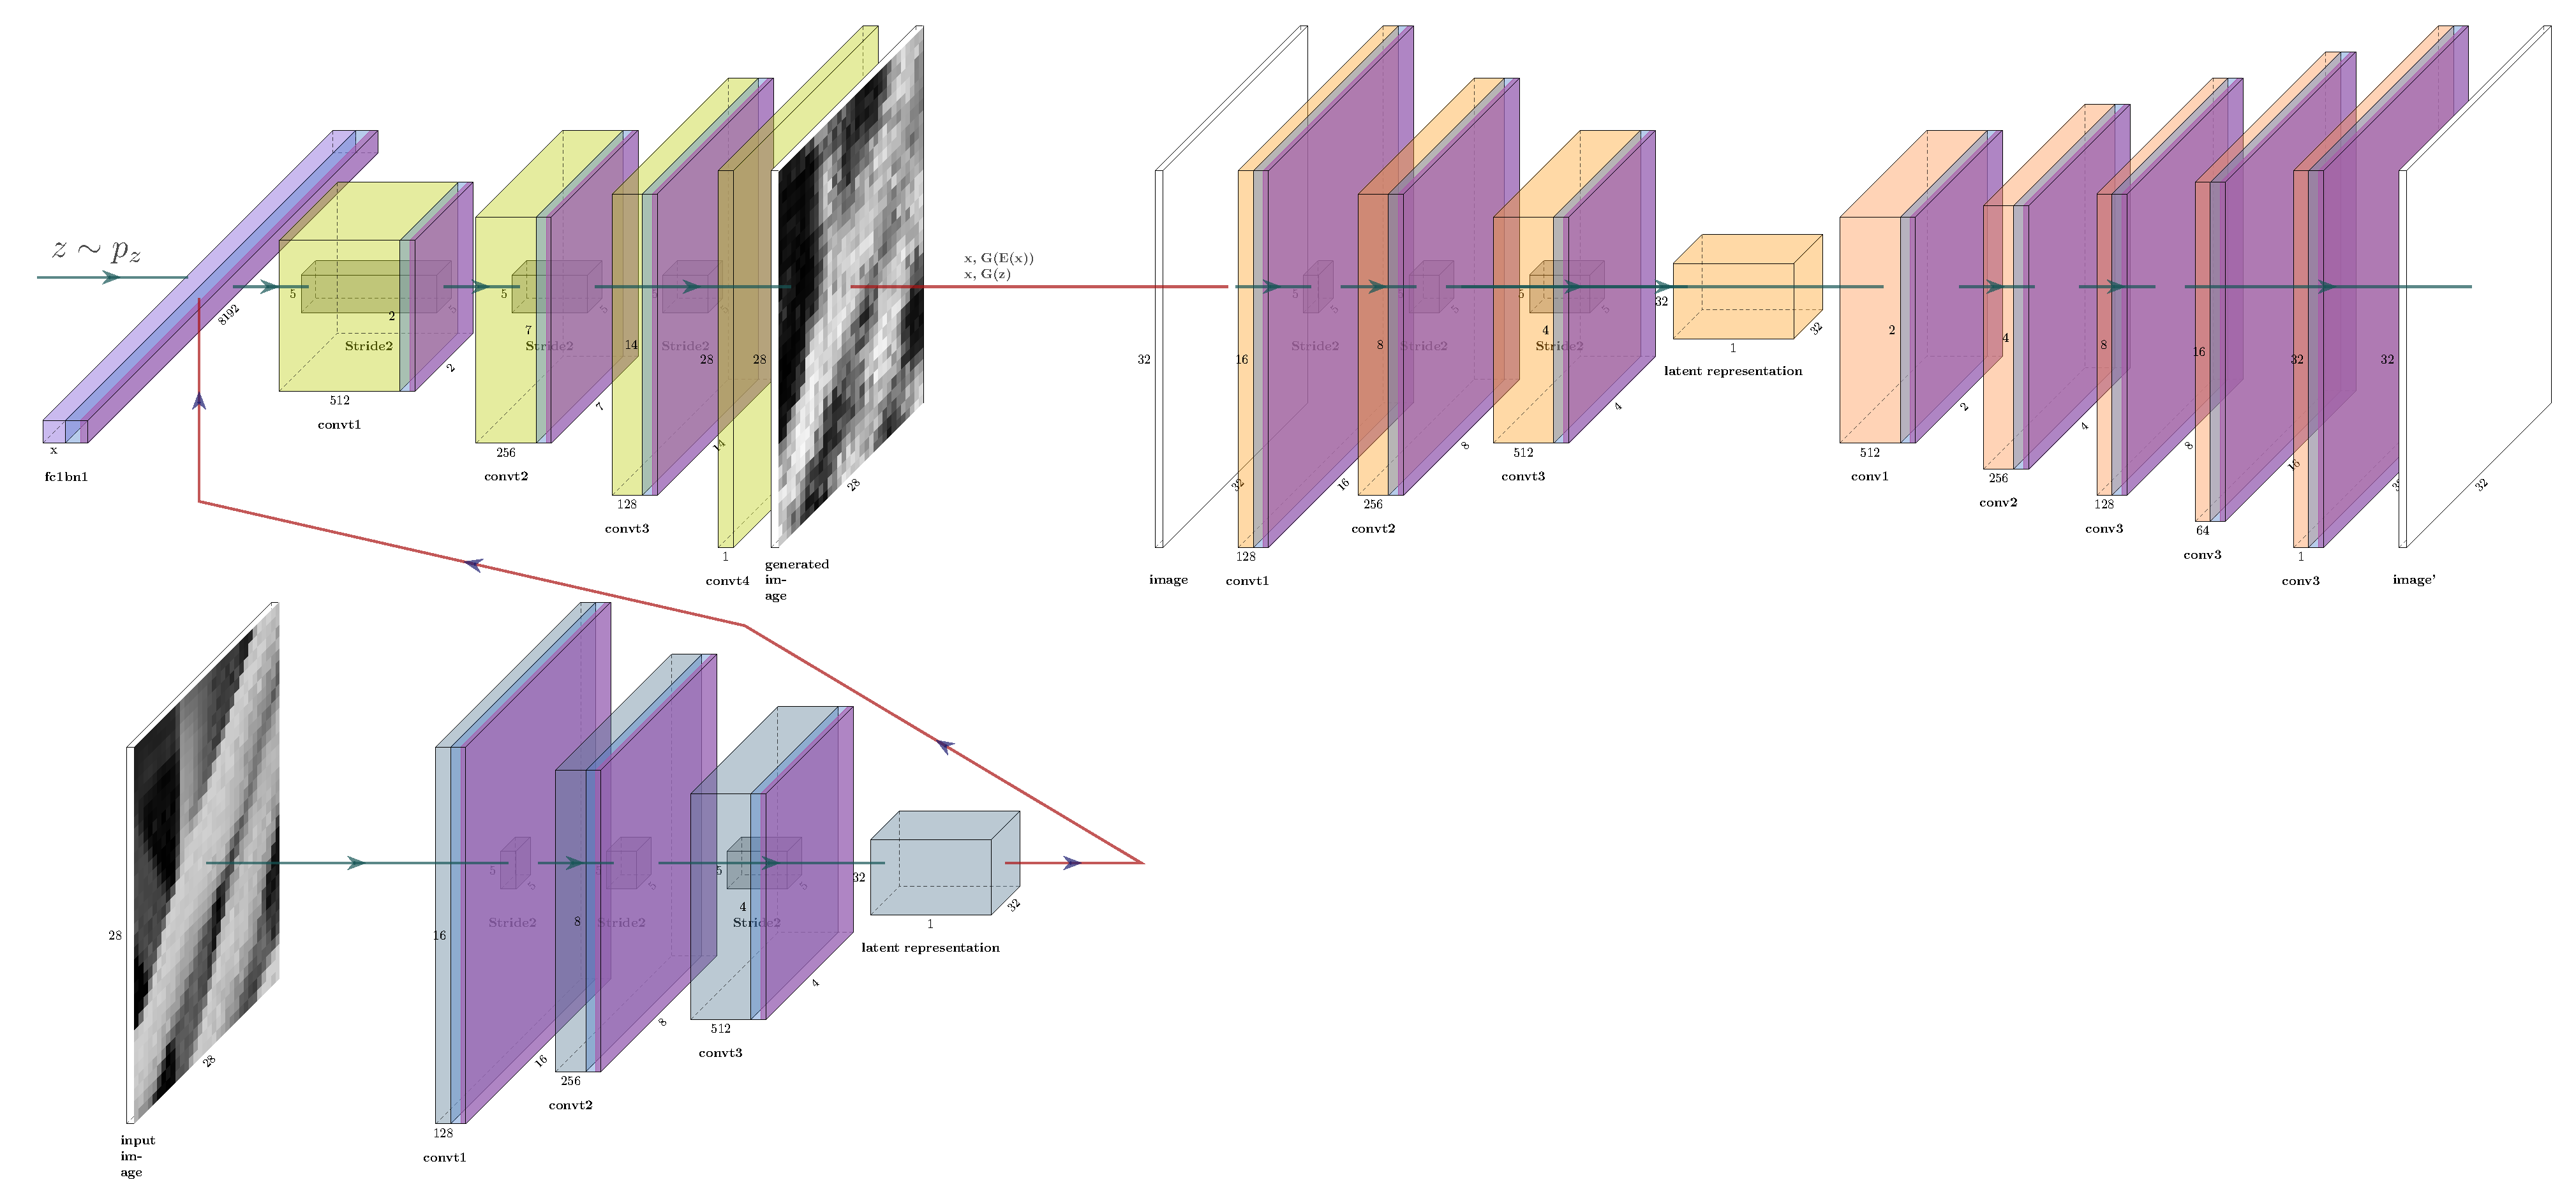
\includegraphics[width=1.0\textwidth]{encebgan}
	\caption{ENCEBGAN Model Overview }
	\label{fig:encebgan_model}
\end{figure}

\section{Sequentially Encoded Energy Based Generative Adversarial Network}
\label{sec:sencebgan}

\begin{figure}[h!]
	\centering
	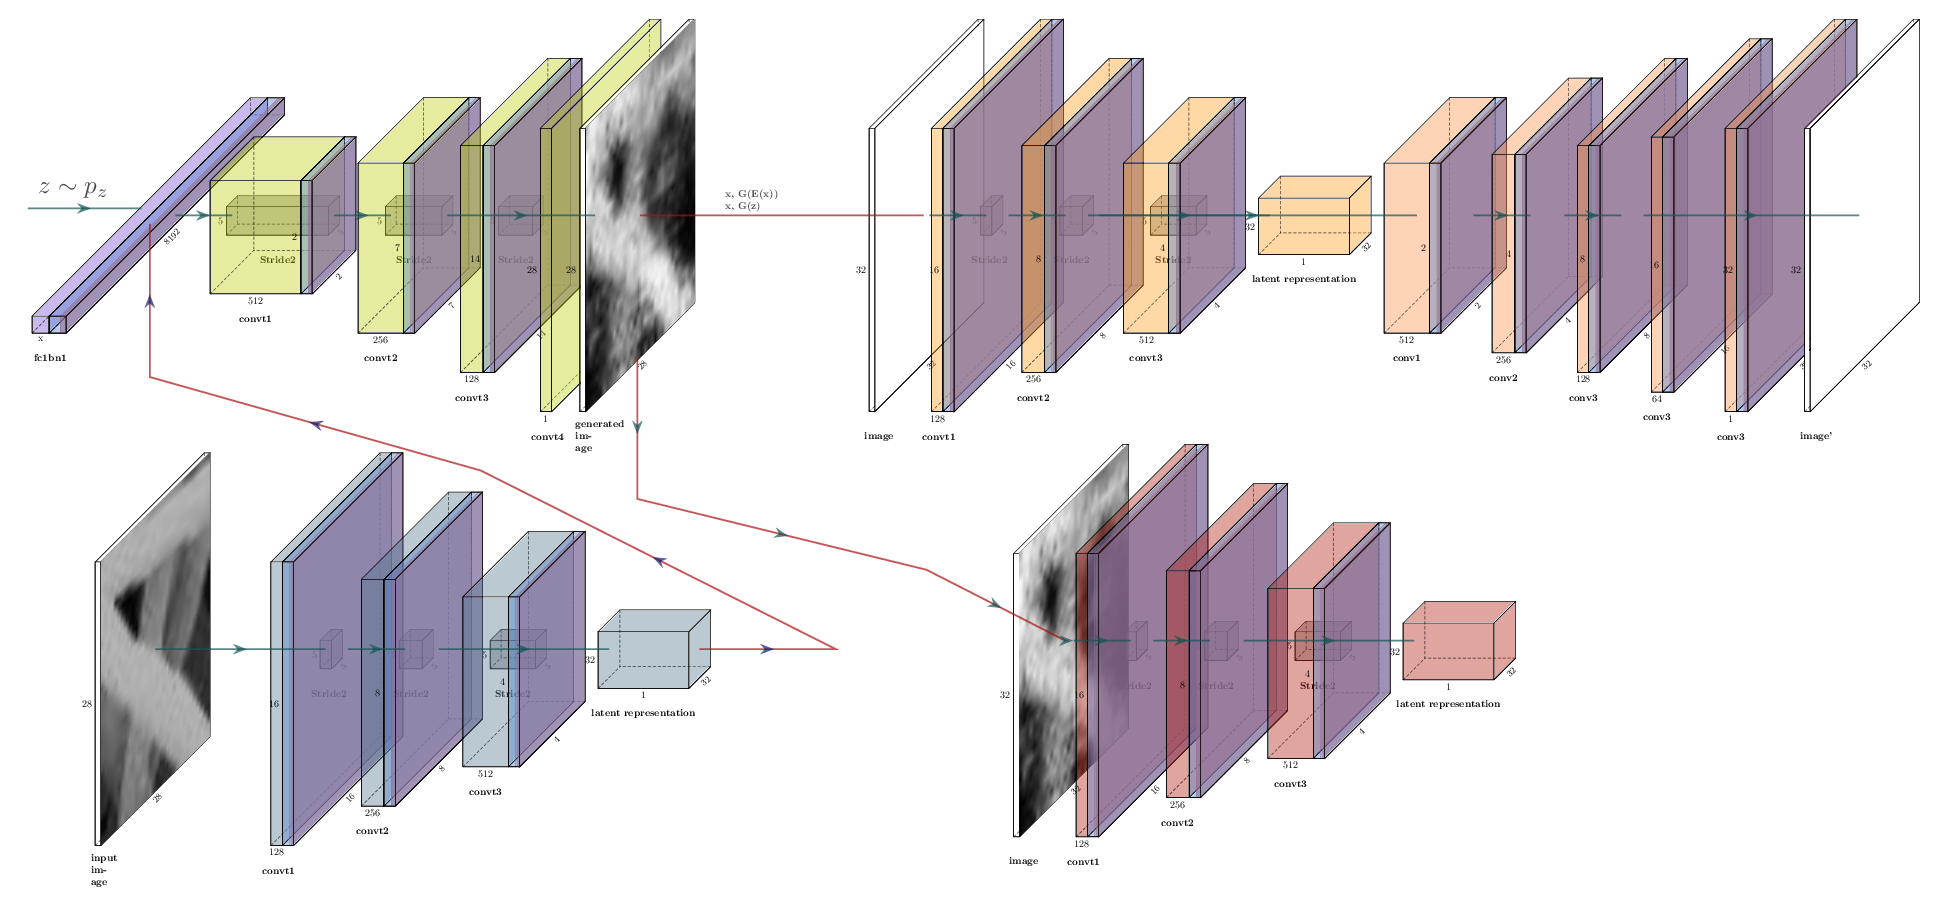
\includegraphics[width=1.0\textwidth]{sencebgan}
	\caption{SENCEBGAN Model Overview }
	\label{fig:sencebgan_model}
\end{figure}

\begin{figure}[h!]
	\centering
	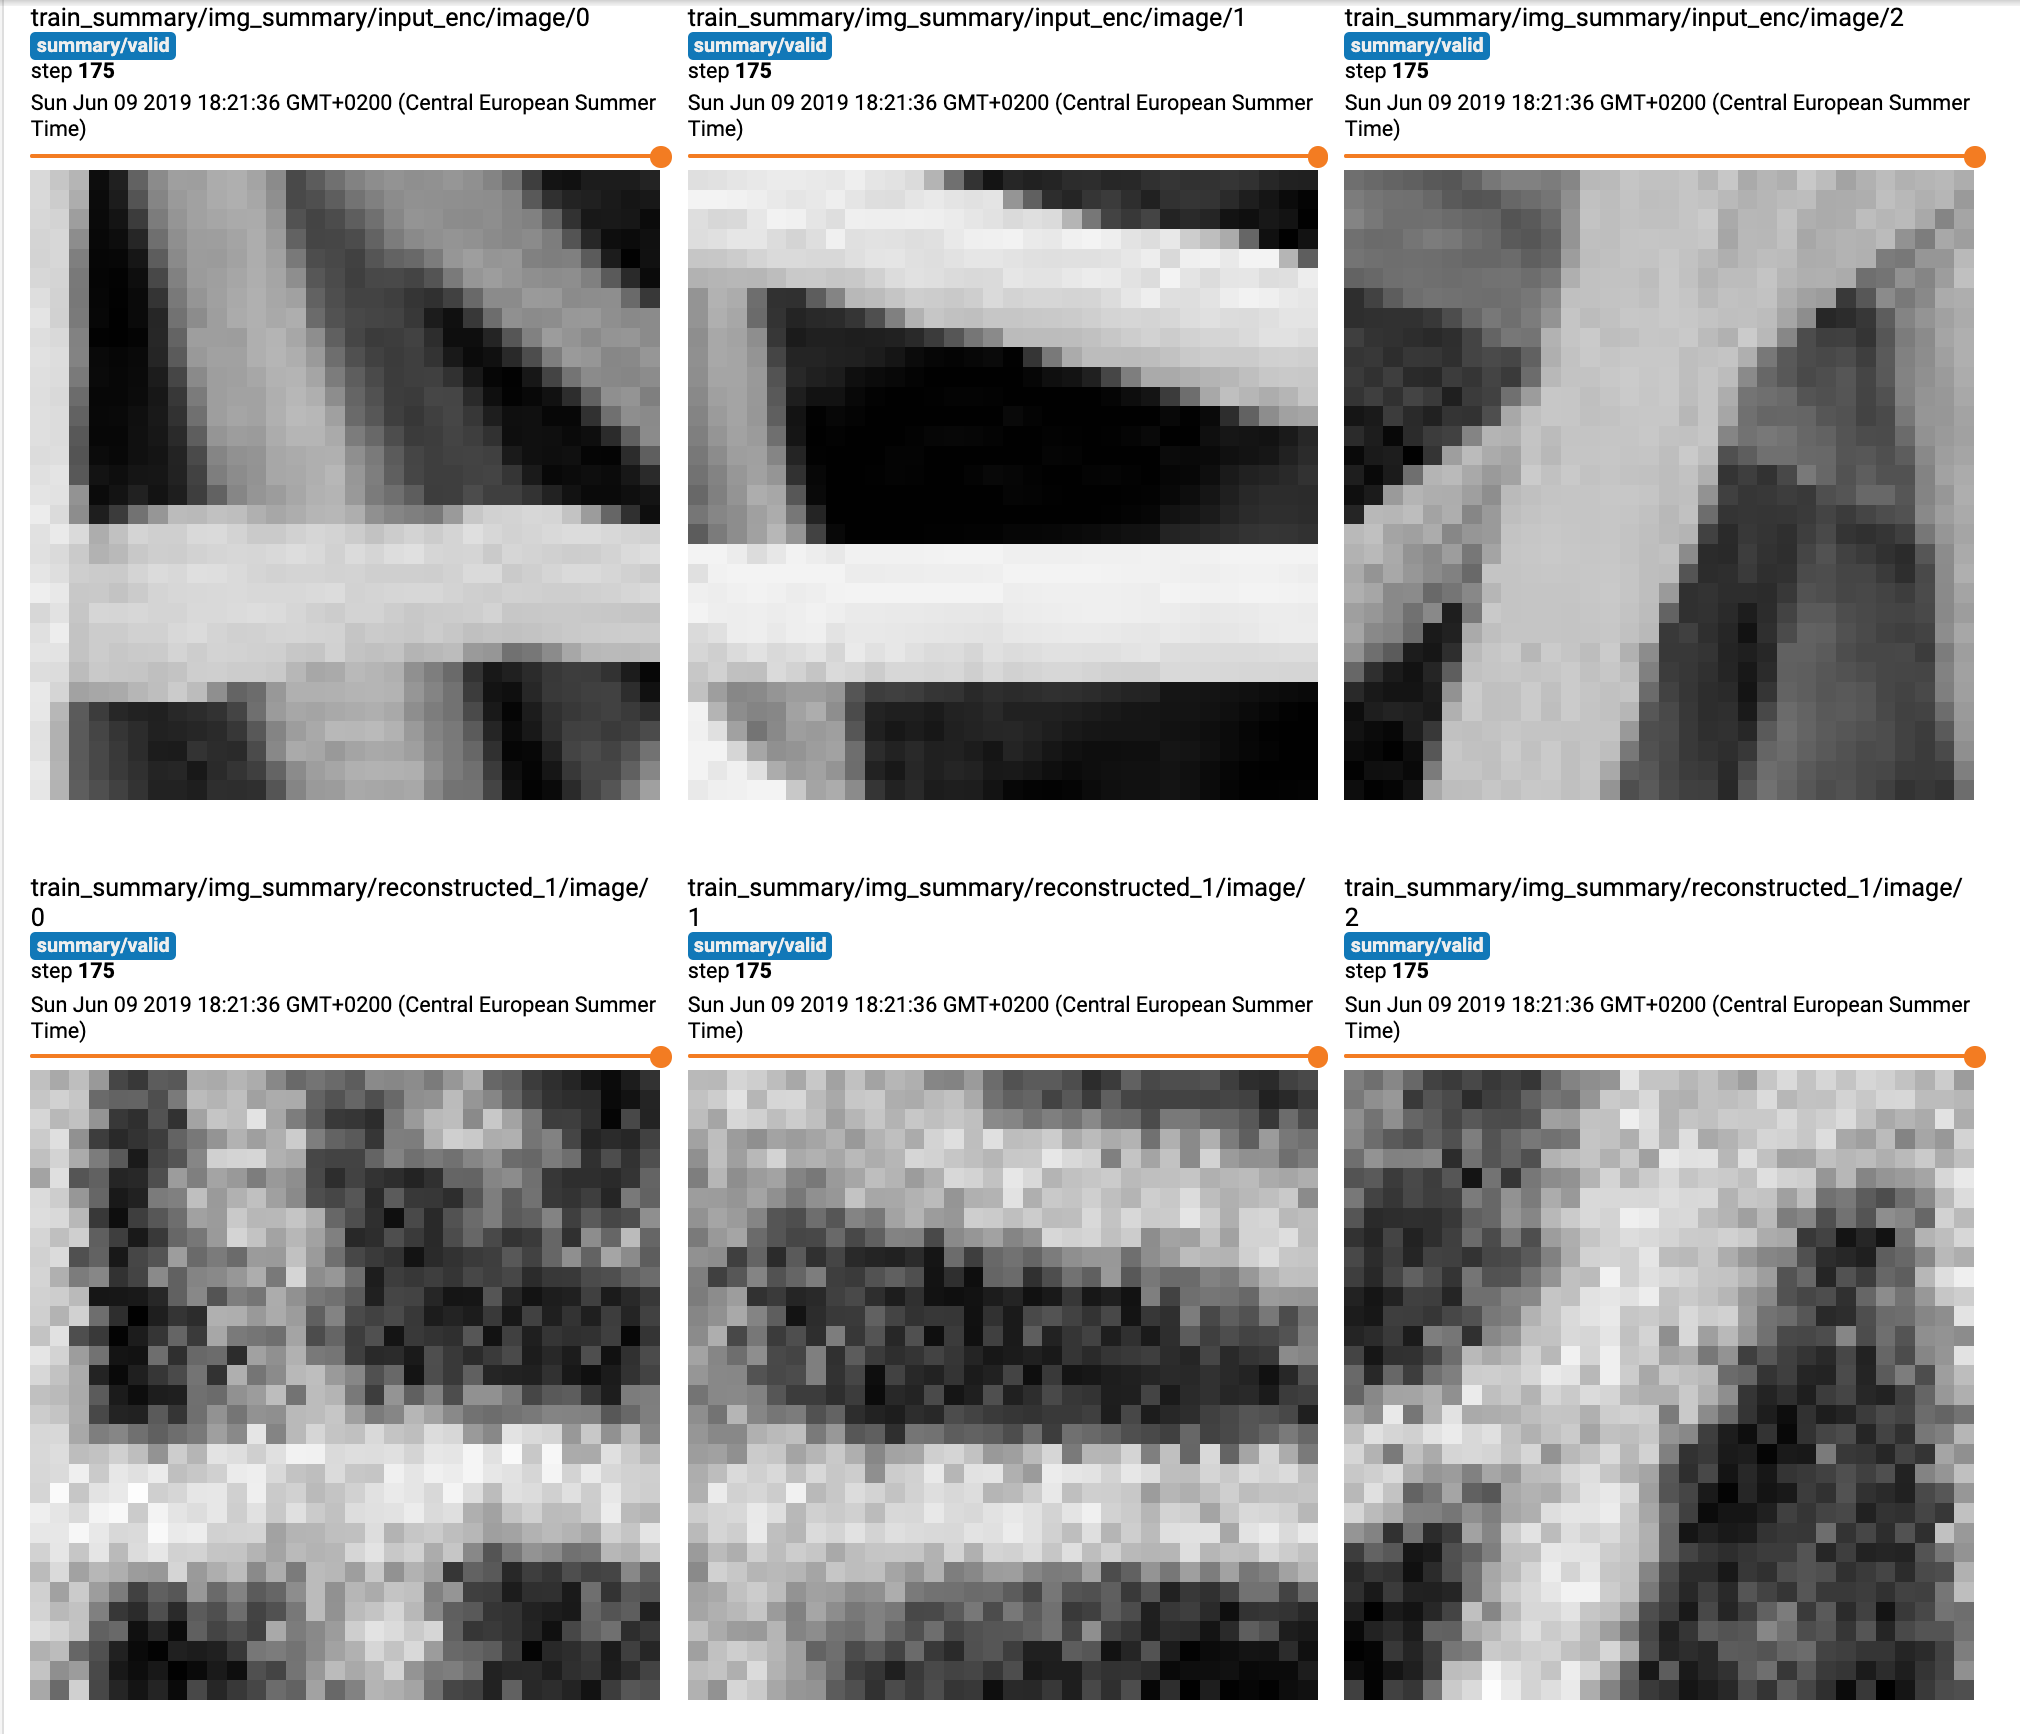
\includegraphics[width=0.75\textwidth]{reconstruct_sencebgan}
	\caption{SENCEBGAN Image Reconstruction  }
	\label{fig:sencebgan_model}
\end{figure}



\endgroup